\section{Análisis}

\subsection{Listado de todas las publicaciones de un autor determinado.}

Para esta query vamos a hacer uso de la potencia que nos ofrece el \textit{aggregation framework}. Este framework funciona creando un pipeline en la que definiremos \textit{stages}. La salida de un \textit{stage} pasa a ser la entrada del \textit{stage} siguiente. Con esto podemos realizar sobre los datos operaciones realmente potentes.

Para obtener el listado de las publicaciones, la query que debemos ejecutar es sencilla. En primer lugar filtramos por el nombre de autor que del cual queremos hacer la consulta, y a continuación concatenamos los \textit{arrays} con los títulos de las publicaciones.

\begin{minted}[
frame=single]{js}
db.authors.aggregate([
  { $match : { _id : "Chin-Wang Tao" } }, 
  { $project: {publication: {$concatArrays: 
    ["$incollections.title", "$articles.title", "$inproceedings.title"]}}
  }
] )
\end{minted}

\subsection{Número de publicaciones de un autor determinado.}

Esta consula es similar a la anterior, pero debemos añadir un paso más en nuestro \textit{pipeline} en el cual contaremos el número de puclicaciones.

\begin{minted}[
frame=single]{js}
db.authors.aggregate([
  { $match : { _id : "Chin-Wang Tao" } }, 
  { $project: {publication: {$concatArrays: 
    ["$incollections.title", "$articles.title", "$inproceedings.title"]}}
  },
  {$project: {number_of_publications: {$size: "$publications"}}}
] )
\end{minted}

\subsection{Número de artículos en revistas para el año 2017.}

\begin{minted}[
frame=single]{js}
db.articles.find({year: 2017}).count()
\end{minted}

Aprovechando que esta query es simple, podemos ver la importancia que adquieren los índices en cuanto a tiempo de ejecución:

\begin{figure}[H]
  \centering
    \centering
        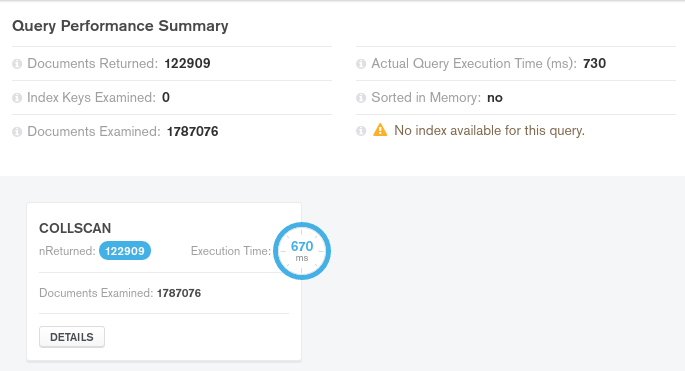
\includegraphics[width=0.4\textwidth]{Figures/wo_year_idx}
        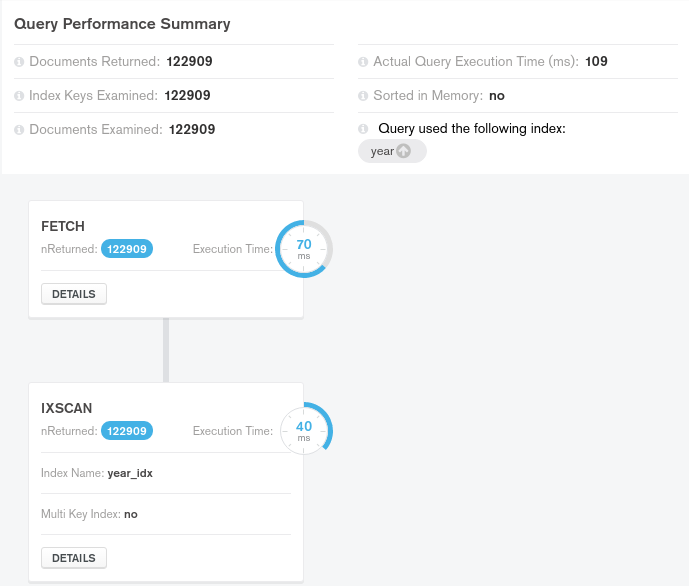
\includegraphics[width=0.4\textwidth]{Figures/year_idx}
  \caption{A la izquierda, la query sin indice, a la derecha, aplicando un índice sobre la columna year.}
\end{figure}

El tiempo de respuesta es casi 7 veces inferior al hacer uso del índice.

\subsection{Número de autores ocasionales (menos de 5 publicaciones).}

En esta ocasión no hará falta hacer uso del \textit{aggregation framework}, si no que haremos una búsqueda utilizando la función \textbf{find()}.

\begin{minted}[
frame=single]{js}
db.authors.find({$expr: {$lt: [{$concatArrays: ["$incollections", "$articles",
  "$inproceedings"]}, 5]}}).count()
\end{minted}

\subsection{Número de artículos y de artículos en congresos de los diez autores con más publicaciones en total.}

Volvemos a usar \textit{aggregation framework} y construimos un \textit{pipeline} con varios pasos. Primero contamos el número de cada tipo de publicacion de cada uno de los autores. A continuación, creamos un nuevo campo con el con \textbf{\$addFields} con el total de publicaciones. Con \textbf{\$sort} y \textbf{\$limit} ordenamos por el campo recién creado y nos quedamos solo con los 10 primeros, es decir, con los autores que más publicaciones tienen. Por último, y con el \textit{stage} \textbf{\$project}, nos quedamos solo con los campos que nos interesan (el campo \textbf{\_id} se incluye por defecto si no se especifica lo contrario).

\begin{minted}[
frame=single]{js}
db.authors.aggregate(
  [
    {$project: {
      "total_incollections": {$size: {$ifNull: ['$incollections', []]},},
      "total_inproceedings": {$size: {$ifNull: ['$inproceedings', []]},},
      "total_articles": {$size: {$ifNull: ['$articles', []]},}
    }},
    {$addFields: {
      "total_publications": { $add: [ "$total_incollections", "$total_inproceedings",
                  "$total_articles" ] }
    }},
    {$sort : { total_publications : -1 } },
    {$limit : 10},
    {$project: {
      "total_articles": 1,
      "total_inproceedings": 1
    )}
  ],
  { allowDiskUse: true }
)
\end{minted}

\subsection{Número medio de autores por publicación.}

En este caso vamos a tener que hacer consulta a varias coleciones y luego hacer calculos con los datos obtenidos en estas consultas.

En primer lugar realizamos consultas en cada una de las colecciones para obtener el número total de autores, incluyendo duplicados. Es decir, si por ejemplo, en un artículo han participado 3 autores, se sumara 3 a la cuenta de autores para esta colección. Estos resultados son sumados y el total lo dividimos por el número total de publicaciones guardadas.

\begin{minted}[
frame=single]{js}
(db.articles.aggregate([
  {$match: {author : {$exists: true}}}, 
  {$project: {num_authors: { $size: '$author' }}}, 
  {$group: {_id: '', num_authors: {$sum: '$num_authors'}}}, 
  {$project: {_id: 0, 'num_authors': '$num_authors'}}])
  .next()['num_authors'] +
db.incollections.aggregate([
  {$match: {author : {$exists: true}}}, 
  {$project: {num_authors: { $size: '$author' }}}, 
  {$group: {_id: '', num_authors: {$sum: '$num_authors'}}}, 
  {$project: {_id: 0, 'num_authors': '$num_authors'}}])
  .next()['num_authors'] +
db.inproceedings.find({author : {$exists: true}}).count())/
(db.articles.find().count() + 
  db.incollections.find().count() + 
  db.inproceedings.find().count())
\end{minted}

\subsection{Lista de coautores de un autor.}

Para poder recuperar esta información, será necesario acceder a cada una de las publicaciones de la lista de publicaciones de un autor, ``seguir'' la referencia para obtener la publicación, y extraer los autores de esta. Para poder ``seguir'' una referencia a otro documento, \textit{aggregation framework} cuenta con el \textit{stage} \textbf{\$lookup}, al que le decimos en que colección buscar y que campos tiene que utilizar a la hora de realizar la busqueda.

\begin{minted}[
frame=single]{js}
db.authors.aggregate([
  { $match : { _id : "Chin-Wang Tao" } },
  {$lookup:
    {
      from: "articles",
      localField: "articles._id",
      foreignField: "_id",
      as: "articles_detail"
    }
  },
  {$lookup:
    {
      from: "incollections",
      localField: "incollections._id",
      foreignField: "_id",
      as: "incollections_detail"
    }
  },
  {$project:{
      _id : 1,
      authors_detail : { $concatArrays: [ "$articles_detail", "$incollections_detail" ] }
    } 
  },
  {$project: {
    "_id": 0,
    "results": {
      $reduce: {
        input: "$authors_detail.author",
        initialValue: [],
        in: { $concatArrays : ["$$value", "$$this"] }
      }
    }
  }
  },
  { $unwind : "$results" },
  {$group: {
    _id: "$results",
    }
  },
  {$group: {
      _id: null,
      coauthors: { $push: { _id: "$_id"} }
    }
  },
  {$project: {
      _id: 0,
      "coauthors": "$coauthors._id"
    }
  }
])
\end{minted}


\subsection{Edad de los 5 autores con el periodo de publicaciones más largo.}

En primer lugar, y usando las facilidades de  \textit{aggregation framework}, agrupamos todas las publicaciones de un mismo autor en una lista única. A continuación nos quedamos de estas listas solo con el año de publicación de estas, y filtramos tanto el máximo como el mínimo de de estos años. Ya con esto, podemos calcular la diferencia entre ambos años y realizar una ordenación a partir de este campo para quedarnos con los cinco primeros.

\begin{minted}[
frame=single]{js}
db.authors.aggregate(
  [
    {$project: {
      publication: {$concatArrays: [
        {$ifNull: ['$incollections', []]},
        {$ifNull: ['$inproceedings', []]},
        {$ifNull: ['$articles', []]}]}
    }},
    {$addFields: {
      max_publication: { $max: "$publication.year"},
      min_publication: { $min: "$publication.year"}
    }},
    {$addFields: {
      age: { $subtract: [ "$max_publication", "$min_publication"] }
    }},
    {$sort : { age : -1 } },
    {$limit : 5},
    {$project: {
      _id: 1,
      age: 1
    }}
  ],
  { allowDiskUse: true }
)
\end{minted}

\subsection{Número de autores novatos.}

Caso idéntico al anterior, cambiando las fases finales para quedarnos con aquellos cuya ``edad'' es inferior a 5 años, y contar el número de elementos que obtenemos.

\begin{minted}[
frame=single]{js}
db.authors.aggregate(
  [
    {$project: {
      publication: {$concatArrays: [
        {$ifNull: ['$incollections', []]},
        {$ifNull: ['$inproceedings', []]},
        {$ifNull: ['$articles', []]}]}
    }},
    {$addFields: {
      max_publication: { $max: "$publication.year"},
      min_publication: { $min: "$publication.year"}
    }},
    {$addFields: {
      "age": { $subtract: [ "$max_publication", "$min_publication"] }
    }},
    {'$match':{'age': {'$lt': 5}}}
  ],
  { allowDiskUse: true }
).itcount()

\end{minted}

\subsection{Porcentaje de publicaciones en revistas con respecto al total de publicaciones.}

Al igual que hicimos cuando calculamos el número medio de autores, que tuvimos que hacer varias queries a cada una de las colecciones, para este caso vamos a volver a operar con diversas queries aplicadas sobre las distintas colecciones. Necesitaremos obtener el número de documentos en cada colección y con estos datos podemos calcular el porcentaje de publicaciones en revistas como número de estas dividido entre el número total de publicaciones.

\begin{minted}[
frame=single]{js}
db.articles.find().count()*100/(
  db.articles.find().count() + 
  db.incollections.find().count() + 
  db.inproceedings.find().count())
\end{minted}
